\chapter{Training Word Embeddings in Arabic}
\label{sec:training}

There are a number of decisions to be made when training word embeddings in Arabic. We have chosen to use the Word2vec framework to train, although there are other proposed methods to obtain word embeddings that are highly similar \cite{pennington2014glove}. We chose Word2vec as there is more public research available for reference as well as excellent open software support. The main decisions to be made when training Word2vec embeddings in Arabic are how to preprocess the text, how to normalize the text, and how to parameterize the Word2vec algorithms. The high level process of training Arabic word embeddings is illustrated in Figure \ref{fig:training}. The remainder of this section describes different consideration for each of these steps, explains options and training parameters that can be adjusted, and presents the specific training parameters we used in our evaluation. 

\begin{figure}
  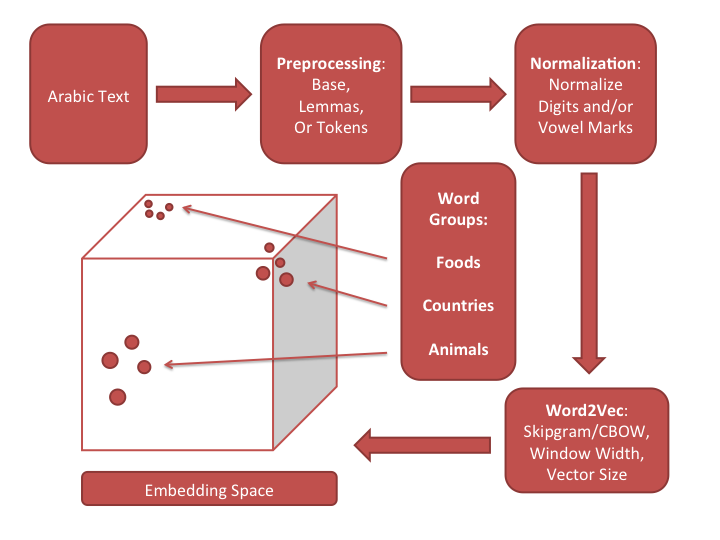
\includegraphics[width=\linewidth]{diagrams/Slide1.png}
  \caption{Training Arabic Word Embeddings}
  \label{fig:training}
\end{figure}

\section{Preprocessing Options}

Preprocessing is very important when analyzing Arabic text. Much of the linguistic information in the grammar is contained in various affixes to words. This is very different from English, where information is often contained in stand-alone pronouns and articles. Word2vec captures information at a word level, so separating these affixes into individual words greatly changes what is learned during training.
\\
The three main preprocessing options that we consider for this task are 1) leave the base text unedited (base), 2) tokenize the text to make affixes individual words (tokens), and 3) lemmatize the text to drop most affixes and preserve only the core idea of each Arabic word (lemmas). Tokenization breaks each word into simple grammatical tokens and creates separate words from affixes such as the definite article and the various pronouns. Lemmatization completely removes such affixes from the corpus, mapping each word to a base word that represents the core meaning of the word. It reduces words to a single tense, gender, and definiteness, but preserves the basic grammatical form. An English equivalent would be to map both \textit{he jumped} and \textit{she jumps} to \textit{he jumps}.

\section{Normalization}

Normalizing Arabic text can greatly reduce the sparsity of the word space in Arabic. We always normalize the corpus by removing English characters, reducing all forms of the letters alif, hamza, and yaa to single general forms (respectively \<ا>,\<ء>,and \<ي>).  The options we consider variable are removing diacritics and reducing both English and Arabic numerical characters to the number sign.

\section{Parameterizations}

The main parameters of Word2vec that are considered are algorithm, embedding dimension, and window size. Both CBOW and Skip-gram algorithms are considered \cite{mikoloveffic:2013}. The defining difference between these methods is that CBOW trains embeddings by attempting to predict a word given its context while Skip-gram tries to predict a word's context given the word. The embedding dimensions considered are 100 and 200. We chose these vector sizes as the typical range is between 100 and 300, where more dimensions require more time and data to train well. We believe we lack sufficient Arabic text data to fully benefit from higher dimensions, so we chose to keep only smaller dimensionalities. The window sizes considered are 4 and 7, which is how far to either side of the word being trained we look for context words. For both the vector sizes and the window widths we were limited to two values for the sake of time. Training models for all combinations of parameters listed above results in 96 models, each requiring well over an hour to train. We believe that our choices provide us with sufficient granularity to understand how Arabic text can be best be used to train high quality word embeddings. For a complete list of the Word2Vec parameter choices, including the static parameters, refer to Table \ref{table:params}. Hierarchical softmax and negative sampling are methods to sample training data efficiently. Downsampling is used to decrease the influence of high frequency words in the corpus. We use hierarchical sampling and some downsampling as together they have been shown to perform well on complex vocabularies with infrequently represented words and phrases \cite{mikolovdist:2013}.

\begin{table}
\begin{center}
\begin{tabular}{l|l|l}
\textbf{Parameter} & \textbf{Value} & \textbf{Explanation} \\
\hline
$sg$ & $[0,1]$ & Algorithm \\
$size$ & $[100, 200]$ & Dimensionality \\
$window$ & $[4, 7]$ & Context window \\
$min count$ & $5$ & Filters rare words \\
$sample$ & $1e-5$ & Downsampling \\
$seed$ & $1$ & Random seed \\
$hs$ & $1$ & Hierarchical softmax \\
$negative$ & $0$ & Negative sampling \\
$iterations$ & $5$ & Training iterations \\
\end{tabular}
\caption{Training Parameters}
\label{table:params}
\end{center}
\end{table}
